\documentclass[convert = false, border=5pt]{standalone}
\usepackage{fontspec}
\setmainfont{Roboto}
\usepackage[siunitx, straightvoltages]{circuitikzgit}
\usepackage{tikz}


\usepackage{amssymb}

\begin{document}
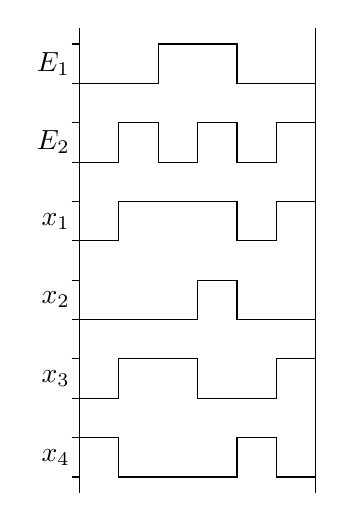
\begin{tikzpicture}
  \draw (0,-.2) -- (0,5.7) (3,-0.2) -- (3,5.7);
  \draw (0,.25) node[anchor=east] {$x_4$} (0,0)  -- ++(-.1,0) ++(0,.5) -- ++(.1,0) (0,.5) -- (0.5,.5) -- (.5,0) -- (2,0) -- (2,.5) -- (2.5,.5) -- (2.5,0) -- (3,0);
  \draw (0,1.25) node[anchor=east] {$x_3$} (0,1) -- ++(-.1,0) ++(0,.5) -- ++(.1,0) ++(0,-.5) -- ++(.5,0) -- ++(0,.5) -- ++(1,0) -- ++(0,-.5) -- ++(1,0) -- ++(0,.5) -- ++(.5,0);
  \draw (0,2.25) node[anchor=east] {$x_2$} (0,2) -- ++(-.1,0) ++(0,.5) -- ++(.1,0) ++(0,-.5) -- ++(1.5,0) -- ++(0,.5) -- ++(.5,0) -- ++(0,-.5) -- ++(1,0);
  \draw (0,3.25) node[anchor=east] {$x_1$} (0,3) -- ++(-.1,0) ++(0,.5) -- ++(.1,0) ++(0,-.5) -- ++(.5,0) -- ++(0,.5) -- ++(1.5,0) -- ++(0,-.5) -- ++(.5,0) -- ++(0,.5) -- ++(.5,0);
  \draw (0,4.25) node[anchor=east] {$E_2$} (0,4) -- ++(-.1,0) ++(0,.5) -- ++(.1,0) ++(0,-.5) -- ++(.5,0) -- ++(0,.5) -- ++(.5,0) -- ++(0,-.5) -- ++(.5,0) -- ++(0,.5) -- ++(.5,0) -- ++(0,-.5) -- ++(.5,0) -- ++(0,.5) -- ++(.5,0);
  \draw (0,5.25) node[anchor=east] {$E_1$} (0,5) -- ++(-.1,0) ++(0,.5) -- ++(.1,0) ++(0,-.5) -- ++(1,0) -- ++(0,.5) -- ++(1,0) -- ++(0,-.5) -- ++(1,0);
\end{tikzpicture}
\end{document}